\documentclass{math}

\usepackage{float}
\usepackage{graphicx}
\usepackage{listings}

\title{Principles of Data Management}
\author{Insert Group Name Here}
\date{August 2018 - December 2018}

\begin{document}

\lstset{basicstyle=\ttfamily\footnotesize,breaklines=true}
\maketitle

\section*{Phase 3 Report}

\subsection*{Description}
This project is designed to be a database for an automotive database owner to
keep track of the sale of vehicles. This includes keeping track of the
transaction amount of each sale, which dealer sold the vehicle, the customer
who bought the vehicle, and the vehicle or vehicles that were sold. To ensure
that the customer, dealer, and vehicle can be identified uniquely, each have
stored attributes that allow for unique identification. In addition
to storing this data our database also can utilize specific commands in order to
show data ranging from sales history to types of vehicles in a dealer’s lot.

\subsection*{Design Decisions}
Our first step in design was the creation of a ER diagram to get an overview on
what relations the database would need. This diagram initially included
dealers, vehicles, customers and sales, with each having an array of different
attributes. These attributes can be seen in the diagram below. The next step in
the process was to create a UI storyboard which was somewhat similar to the ER
diagram. The UI design was initiated here in order to get an idea of how the
application itself would function. This diagram gives an overview of the basic
requirements for the project, and was created to be simple and show all actions
that could be taken by a given user. \par
With phase two came an updated ER diagram. Improvements included adding more
attributes in order to better represent necessary values in the table. We also
improved representation of entities this way. The last change we made to our
model was to split up brands into its own entity instead of being an attribute
in vehicle. This enabled a better representation of brand and allowed us to
include more attributes without adding redundant data into the database. With
this phase came the need for a UML diagram to show how the application would
work at a more precise level. This helped us visualize how the different
objects and their functions interacted in the application.

\subsection*{Current Design}
Our current design is split into five main entities:
\begin{itemize}
  \item Vehicles
  \item Brands
  \item Dealers
  \item Sales
  \item Customers
\end{itemize}
These entities all have many attributes that store information relevant to the
object they represent. In order to save space, the ER diagram is presented
below and shows the attributes in each entity and the relations between these
entities. The important attributes and descriptions of the relations are
described here.
\begin{figure}[H]
  \centering
  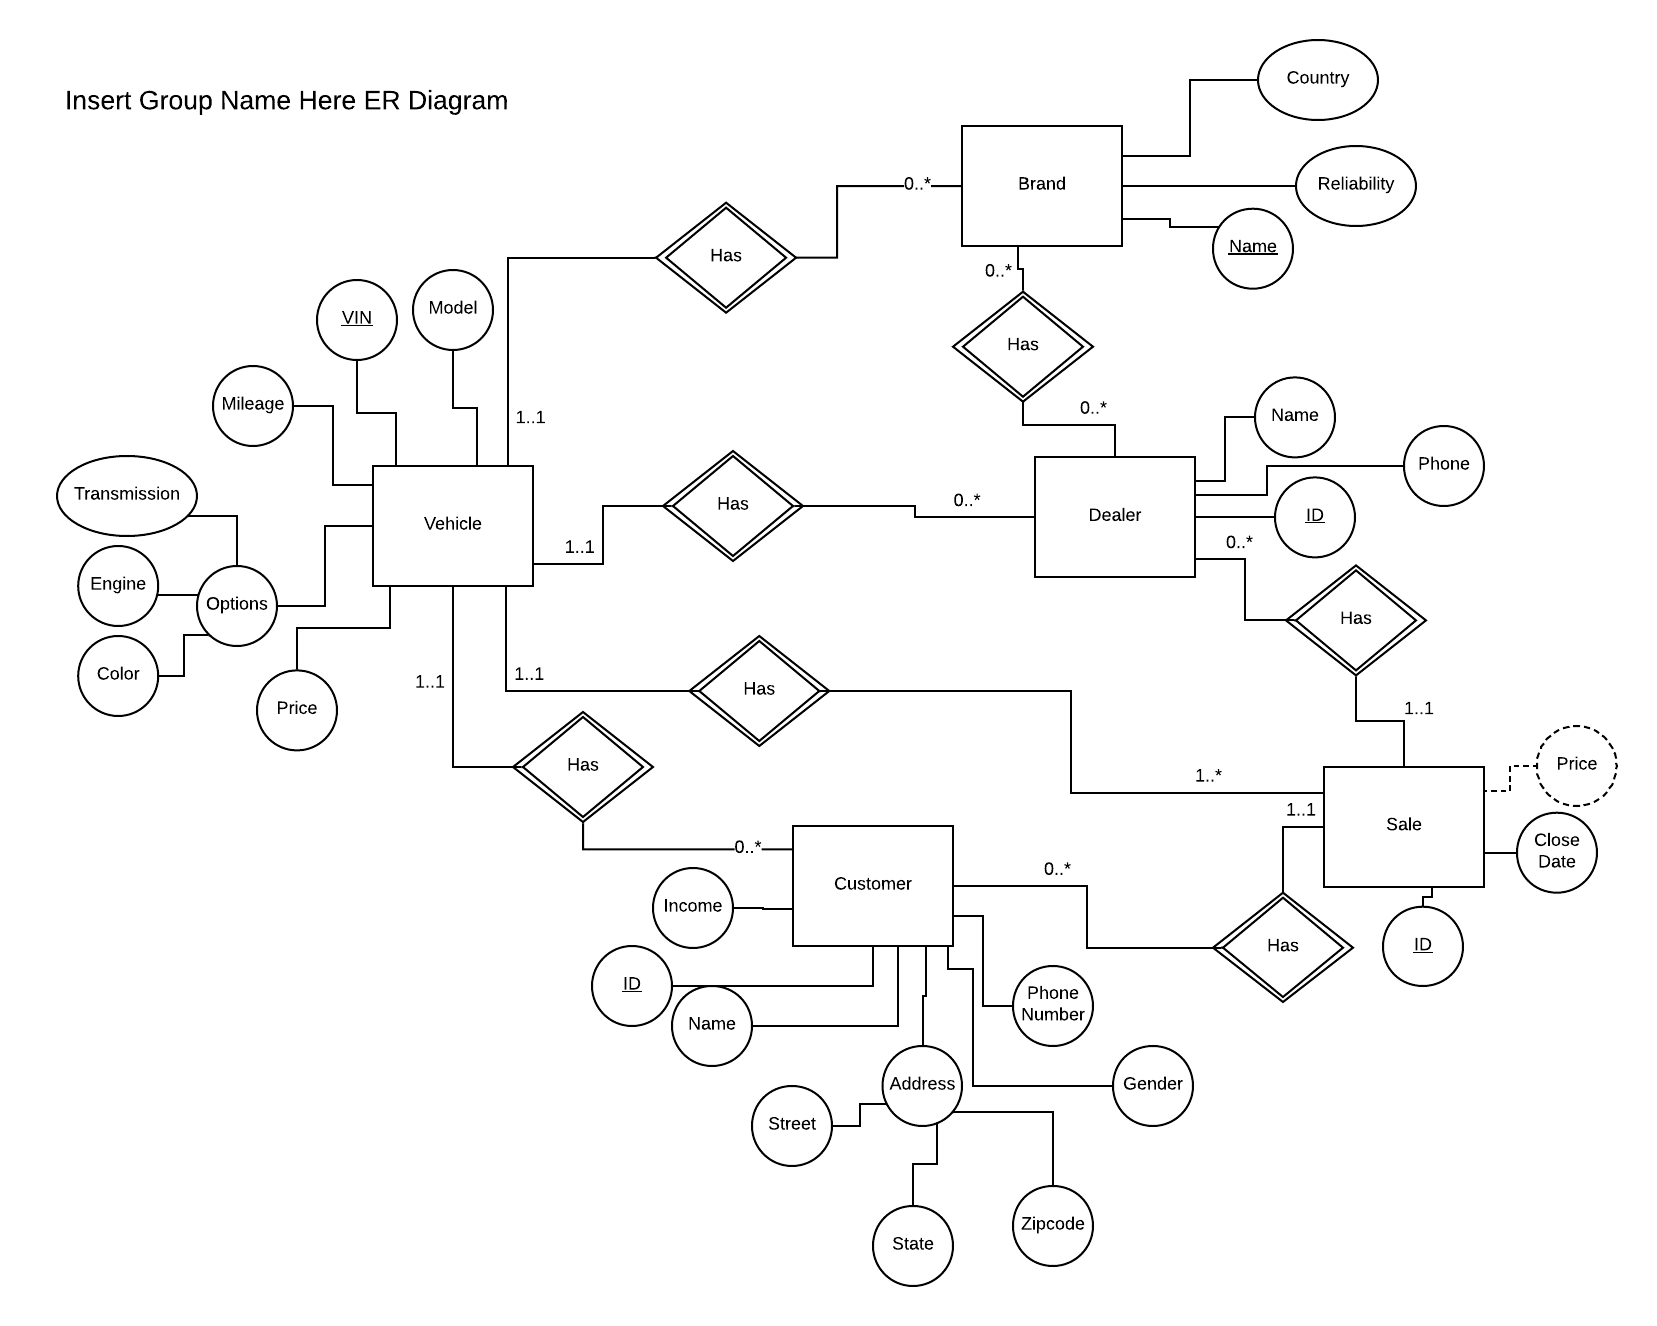
\includegraphics[width=16cm]{assets/phase3_er_diagram.png}
  \caption{Phase 3 ER Diagram}
\end{figure}

\subsection*{SQL Examples}
Below is an example one of the more complex SQL queries present in the project.
\begin{lstlisting}
select v.sale as id, d.name as dealer, c.name as customer,
  s.close_date, sum(v.price) as price from
  vehicles v inner join dealers d on v.dealer = d.id inner join
    customers c on v.owner = c.id inner join
    sales s on s.id = v.sale
  where d.id=$1
  group by v.sale, d.name, c.name, s.close_date
  order by s.close_date
\end{lstlisting}
This code is meant to get the total value of a sale by summing up the price of
the vehicles in the sale. It does this by performing an inner join across the
sales, customers, dealers, and vehicles table to match together and aggregate
all the relevant information.

\subsection*{Application Design}
This project required us to make many choices pertaining to the design of
our application. Two early decisions that were interwoven were our choice of
programming language and interface. We first decided to use a Command Line
Interface, due to the experience of our group with such interfaces, and its ease
of setup compared to a GUI. For our language, we chose node.js because of
language familiarity and the rich package ecosystem. For this project, we used
the following packages to speed up development:
\begin{itemize}
  \item \texttt{yargs.js} to perform argument parsing and organize the
    structure of the CLI
  \item \texttt{cli-table3} to format query outputs into terminal friendly
    tables
  \item \texttt{colors.js} to color the output using terminal friendly ANSI
    color codes
  \item \texttt{pg} (node-postgres) as a way to interface node.js with our
    postgres database
  \item \texttt{underscore} as a lightweight utility library
\end{itemize}

\subsubsection*{Example Command}
\begin{figure}[H]
  \centering
  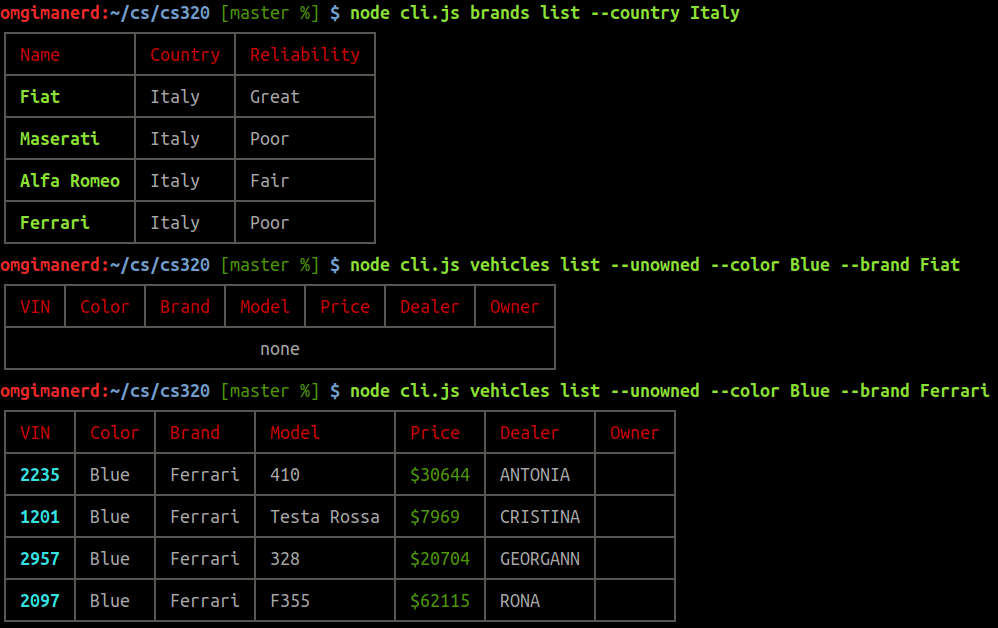
\includegraphics[width=16cm]{assets/phase3_example_command.png}
  \caption{Example Command Invocations}
\end{figure}
Another design decision we made was to prevent the deletion of records from the
database via the application. We decided to treat all entries to the database as
permanent, and therefore there are no provided commands for users to do so.
We made this design decision because many of our records reference other
elements in the database, and allowing deletions would result in missing data.
For example, if a user deletes a car because the car is totaled, the dealer who
sold the car would no longer know what car they sold in that sale, even though
they would still know what customer they sold the car too. \par
Most of the heavy lifting and business logic in the CLI is performed by
complex SQL queries executed on the database. The CLI merely serves to
construct the queries with the proper parameters and display the subsequent
results.

\subsection*{User Actions}
Our application allows users to conduct a variety of actions. A user can add,
update, or list the following:
\begin{itemize}
  \item car brands
  \item customers
  \item dealers
  \item sales
  \item vehicles
\end{itemize}
Dealers have two attributes which must be specified by a user, name and phone
number. Dealers can be added by invoking:
\begin{lstlisting}
node cli.js dealer add <name> <phone>
\end{lstlisting}
Similarly, the syntax for adding a brand is:
\begin{lstlisting}
node cli.js add <name> <country> <reliability>
\end{lstlisting}
The name is the primary key of the brand and must be unique. For listing out
entities, there are a variety of flags the user can include to filter their
search. These flags can be viewed by invoking the \texttt{--help} flag on any
command in the CLI.

\subsection*{Overall Project Progress}
We started out disorganized at first by talking mainly through email, and this
caused some problems. These included not replying back to everyone (resulting
in a late submission) and having an awkwardly long email chain. This problem
eventually was solved once we switched over to Slack as this made group
messaging and sharing of diagrams and documents back and forth much easier, in
a cleaner format. The next phase went much smoother, as we started with ample
time and were able to complete most of the requirements quicky, with only a few
problems with design requirements. These were quickly resolved with
consultation of the given documents and by asking questions and discussing
within our team. For our last phase our main problem was creation of sample
code using a python script and making sure our diagrams matched our
implementation. This issues were quickly resolved through efficient
communication.

\subsection*{Contributions}
Alvin Lin: Responsible for good portion of the command line interface and
underlying SQL, as well as generation of data. \\
Andrew Chabot: Also helped with the database code and creating sample data to
be used in csv and sql files, as well as ER and UMl diagram creation. \\
William Anderson: Worked on the reports as well as other tasks as need be. \\
Jake Edom: Worked primarily on the reports and set up the team slack channel,
helped keep team on task.

\end{document}
